\chapter{Square root algorithms}

\index{square root algorithm}

A \key{square root algorithm} is an algorithm
that has a square root in its time complexity.
A square root can be seen as a ''poor man's logarithm'':
the complexity $O(\sqrt n)$ is better than $O(n)$
but worse than $O(\log n)$.
In any case, many square root algorithms are fast and usable in practice.

As an example, consider the problem of
creating a data structure that supports
two operations on an array:
modifying an element at a given position
and calculating the sum of elements in the given range.
We have previously solved the problem using
binary indexed and segment trees,
that support both operations in $O(\log n)$ time.
However, now we will solve the problem
in another way using a square root structure
that allows us to modify elements in $O(1)$ time
and calculate sums in $O(\sqrt n)$ time.

The idea is to divide the array into \emph{blocks}
of size $\sqrt n$ so that each block contains
the sum of elements inside the block.
For example, an array of 16 elements will be
divided into blocks of 4 elements as follows:

\begin{center}
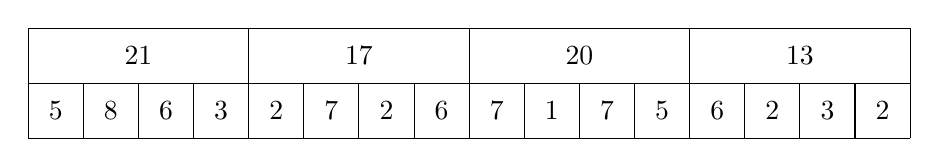
\begin{tikzpicture}[scale=0.7]
\draw (0,0) grid (16,1);

\draw (0,1) rectangle (4,2);
\draw (4,1) rectangle (8,2);
\draw (8,1) rectangle (12,2);
\draw (12,1) rectangle (16,2);

\node at (0.5, 0.5) {5};
\node at (1.5, 0.5) {8};
\node at (2.5, 0.5) {6};
\node at (3.5, 0.5) {3};
\node at (4.5, 0.5) {2};
\node at (5.5, 0.5) {7};
\node at (6.5, 0.5) {2};
\node at (7.5, 0.5) {6};
\node at (8.5, 0.5) {7};
\node at (9.5, 0.5) {1};
\node at (10.5, 0.5) {7};
\node at (11.5, 0.5) {5};
\node at (12.5, 0.5) {6};
\node at (13.5, 0.5) {2};
\node at (14.5, 0.5) {3};
\node at (15.5, 0.5) {2};

\node at (2, 1.5) {21};
\node at (6, 1.5) {17};
\node at (10, 1.5) {20};
\node at (14, 1.5) {13};

\end{tikzpicture}
\end{center}

In this structure,
it is easy to modify array elements,
because it is only needed to update
the sum of a single block
after each modification,
which can be done in $O(1)$ time.
For example, the following picture shows
how the value of an element and
the sum of the corresponding block change:

\begin{center}
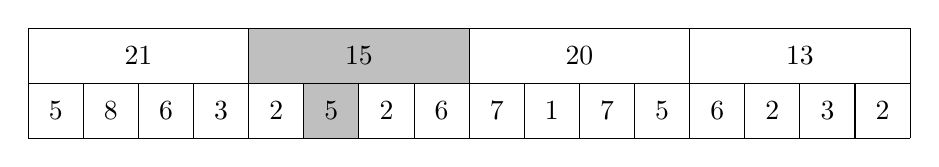
\begin{tikzpicture}[scale=0.7]
\fill[color=lightgray] (5,0) rectangle (6,1);
\draw (0,0) grid (16,1);

\fill[color=lightgray] (4,1) rectangle (8,2);
\draw (0,1) rectangle (4,2);
\draw (4,1) rectangle (8,2);
\draw (8,1) rectangle (12,2);
\draw (12,1) rectangle (16,2);

\node at (0.5, 0.5) {5};
\node at (1.5, 0.5) {8};
\node at (2.5, 0.5) {6};
\node at (3.5, 0.5) {3};
\node at (4.5, 0.5) {2};
\node at (5.5, 0.5) {5};
\node at (6.5, 0.5) {2};
\node at (7.5, 0.5) {6};
\node at (8.5, 0.5) {7};
\node at (9.5, 0.5) {1};
\node at (10.5, 0.5) {7};
\node at (11.5, 0.5) {5};
\node at (12.5, 0.5) {6};
\node at (13.5, 0.5) {2};
\node at (14.5, 0.5) {3};
\node at (15.5, 0.5) {2};

\node at (2, 1.5) {21};
\node at (6, 1.5) {15};
\node at (10, 1.5) {20};
\node at (14, 1.5) {13};

\end{tikzpicture}
\end{center}

Then, to calculate the sum of elements in a range,
we divide the range into three parts such that 
the sum consists of values of single elements
and sums of blocks between them:

\begin{center}
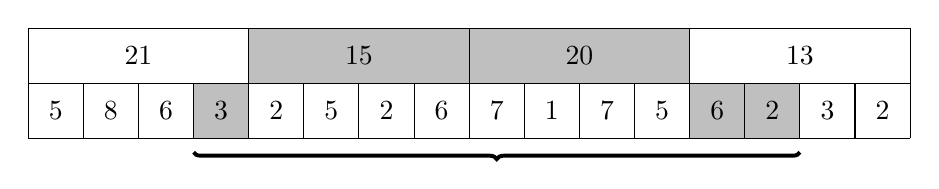
\begin{tikzpicture}[scale=0.7]
\fill[color=lightgray] (3,0) rectangle (4,1);
\fill[color=lightgray] (12,0) rectangle (13,1);
\fill[color=lightgray] (13,0) rectangle (14,1);
\draw (0,0) grid (16,1);

\fill[color=lightgray] (4,1) rectangle (8,2);
\fill[color=lightgray] (8,1) rectangle (12,2);
\draw (0,1) rectangle (4,2);
\draw (4,1) rectangle (8,2);
\draw (8,1) rectangle (12,2);
\draw (12,1) rectangle (16,2);

\node at (0.5, 0.5) {5};
\node at (1.5, 0.5) {8};
\node at (2.5, 0.5) {6};
\node at (3.5, 0.5) {3};
\node at (4.5, 0.5) {2};
\node at (5.5, 0.5) {5};
\node at (6.5, 0.5) {2};
\node at (7.5, 0.5) {6};
\node at (8.5, 0.5) {7};
\node at (9.5, 0.5) {1};
\node at (10.5, 0.5) {7};
\node at (11.5, 0.5) {5};
\node at (12.5, 0.5) {6};
\node at (13.5, 0.5) {2};
\node at (14.5, 0.5) {3};
\node at (15.5, 0.5) {2};

\node at (2, 1.5) {21};
\node at (6, 1.5) {15};
\node at (10, 1.5) {20};
\node at (14, 1.5) {13};

\draw [decoration={brace}, decorate, line width=0.5mm] (14,-0.25) -- (3,-0.25);

\end{tikzpicture}
\end{center}

Since the number of single elements is $O(\sqrt n)$
and the number of blocks is also $O(\sqrt n)$,
the sum query takes $O(\sqrt n)$ time.
The purpose of the block size $\sqrt n$ is
that it \emph{balances} two things:
the array is divided into $\sqrt n$ blocks,
each of which contains $\sqrt n$ elements.

In practice, it is not necessary to use the
exact value of $\sqrt n$ as a parameter,
and instead we may use parameters $k$ and $n/k$ where $k$ is
different from $\sqrt n$.
The optimal parameter depends on the problem and input.
For example, if an algorithm often goes
through the blocks but rarely inspects
single elements inside the blocks,
it may be a good idea to divide the array into
$k < \sqrt n$ blocks, each of which contains $n/k > \sqrt n$
elements.

\section{Combining algorithms}

In this section we discuss two square root algorithms
that are based on combining two algorithms into one algorithm.
In both cases, we could use either of the algorithms
without the other
and solve the problem in $O(n^2)$ time.
However, by combining the algorithms, the running
time is only $O(n \sqrt n)$.

\subsubsection{Case processing}

Suppose that we are given a two-dimensional
grid that contains $n$ cells.
Each cell is assigned a letter,
and our task is to find two cells
with the same letter whose distance is minimum,
where the distance between cells
$(x_1,y_1)$ and $(x_2,y_2)$ is $|x_1-x_2|+|y_1-y_2|$.
For example, consider the following grid:

\begin{center}
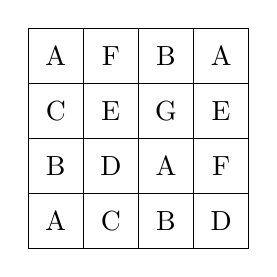
\begin{tikzpicture}[scale=0.7]
\node at (0.5,0.5) {A};
\node at (0.5,1.5) {B};
\node at (0.5,2.5) {C};
\node at (0.5,3.5) {A};
\node at (1.5,0.5) {C};
\node at (1.5,1.5) {D};
\node at (1.5,2.5) {E};
\node at (1.5,3.5) {F};
\node at (2.5,0.5) {B};
\node at (2.5,1.5) {A};
\node at (2.5,2.5) {G};
\node at (2.5,3.5) {B};
\node at (3.5,0.5) {D};
\node at (3.5,1.5) {F};
\node at (3.5,2.5) {E};
\node at (3.5,3.5) {A};
\draw (0,0) grid (4,4);
\end{tikzpicture}
\end{center}
In this case, the minimum distance is 2 between the two 'E' letters.

We can solve the problem by considering each letter separately.
Using this approach, the new problem is to calculate
the minimum distance
between two cells with a \emph{fixed} letter $c$.
We focus on two algorithms for this:

\emph{Algorithm 1:} Go through all pairs of cells with letter $c$,
and calculate the minimum distance between such cells.
This will take $O(k^2)$ time where $k$ is the number of cells with letter $c$.

\emph{Algorithm 2:} Perform a breadth-first search that simultaneously
starts at each cell with letter $c$. The minimum distance between
two cells with letter $c$ will be calculated in $O(n)$ time.

One way to solve the problem is to choose either of the
algorithms and use it for all letters.
If we use Algorithm 1, the running time is $O(n^2)$,
because all cells may contain the same letter,
and in this case $k=n$.
Also if we use Algorithm 2, the running time is $O(n^2)$,
because all cells may have different letters,
and in this case $n$ searches are needed.

However, we can \emph{combine} the two algorithms and
use different algorithms for different letters
depending on how many times each letter appears in the grid.
Assume that a letter $c$ appears $k$ times.
If $k \le \sqrt n$, we use Algorithm 1, and if $k > \sqrt n$,
we use Algorithm 2.
It turns out that by doing this, the total running time
of the algorithm is only $O(n \sqrt n)$.

First, suppose that we use Algorithm 1 for a letter $c$.
Since $c$ appears at most $\sqrt n$ times in the grid,
we compare each cell with letter $c$ $O(\sqrt n)$ times
with other cells.
Thus, the time used for processing all such cells is $O(n \sqrt n)$.
Then, suppose that we use Algorithm 2 for a letter $c$.
There are at most $\sqrt n$ such letters,
so processing those letters also takes $O(n \sqrt n)$ time.

\subsubsection{Batch processing}

Our next problem also deals with
a two-dimensional grid that contains $n$ cells.
Initially, each cell except one is white.
We perform $n-1$ operations, each of which first
calculates the minimum distance from a given white cell
to a black cell, and then paints the white cell black.

For example, consider the following operation:

\begin{center}
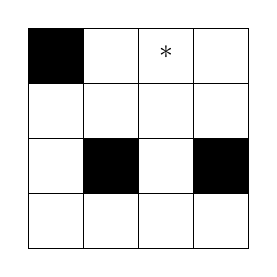
\begin{tikzpicture}[scale=0.7]
\fill[color=black] (1,1) rectangle (2,2);
\fill[color=black] (3,1) rectangle (4,2);
\fill[color=black] (0,3) rectangle (1,4);
\node at (2.5,3.5) {*};
\draw (0,0) grid (4,4);
\end{tikzpicture}
\end{center}

First, we calculate the minimum distance
from the white cell marked with * to a black cell.
The minimum distance is 2, because we can move
two steps left to a black cell.
Then, we paint the white cell black:

\begin{center}
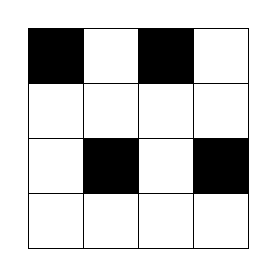
\begin{tikzpicture}[scale=0.7]
\fill[color=black] (1,1) rectangle (2,2);
\fill[color=black] (3,1) rectangle (4,2);
\fill[color=black] (0,3) rectangle (1,4);
\fill[color=black] (2,3) rectangle (3,4);
\draw (0,0) grid (4,4);
\end{tikzpicture}
\end{center}

Consider the following two algorithms:

\emph{Algorithm 1:} Use breadth-first search
to calculate
for each white cell the distance to the nearest black cell.
This takes $O(n)$ time, and after the search,
we can find the minimum distance from any white cell
to a black cell in $O(1)$ time.

\emph{Algorithm 2:} Maintain a list of cells that have been
painted black, go through this list at each operation
and then add a new cell to the list.
An operation takes $O(k)$ time where $k$ is the length of the list.

We combine the above algorithms by
dividing the operations into
$O(\sqrt n)$ \emph{batches}, each of which consists
of $O(\sqrt n)$ operations.
At the beginning of each batch,
we perform Algorithm 1.
Then, we use Algorithm 2 to process the operations
in the batch.
We clear the list of Algorithm 2 between
the batches.
At each operation,
the minimum distance to a black cell
is either the distance calculated by Algorithm 1
or the distance calculated by Algorithm 2.

The resulting algorithm works in
$O(n \sqrt n)$ time.
First, Algorithm 1 is performed $O(\sqrt n)$ times,
and each search works in $O(n)$ time.
Second, when using Algorithm 2 in a batch,
the list contains $O(\sqrt n)$ cells
(because we clear the list between the batches)
and each operation takes $O(\sqrt n)$ time.

\section{Integer partitions}

Some square root algorithms are based on
the following observation:
if a positive integer $n$ is represented as
a sum of positive integers,
such a sum always contains at most
$O(\sqrt n)$ \emph{distinct} numbers.
The reason for this is that to construct
a sum that contains a maximum number of distinct
numbers, we should choose \emph{small} numbers.
If we choose the numbers $1,2,\ldots,k$,
the resulting sum is
\[\frac{k(k+1)}{2}.\]
Thus, the maximum amount of distinct numbers is $k = O(\sqrt n)$.
Next we will discuss two problems that can be solved
efficiently using this observation.

\subsubsection{Knapsack}

Suppose that we are given a list of integer weights
whose sum is $n$.
Our task is to find out all sums that can be formed using
a subset of the weights. For example, if the weights are
$\{1,3,3\}$, the possible sums are as follows:

\begin{itemize}[noitemsep]
\item $0$ (empty set)
\item $1$
\item $3$
\item $1+3=4$
\item $3+3=6$
\item $1+3+3=7$
\end{itemize}

Using the standard knapsack approach (see Chapter 7.4),
the problem can be solved as follows:
we define a function $\texttt{possible}(x,k)$ whose value is 1
if the sum $x$ can be formed using the first $k$ weights,
and 0 otherwise.
Since the sum of the weights is $n$,
there are at most $n$ weights and
all values of the function can be calculated
in $O(n^2)$ time using dynamic programming.

However, we can make the algorithm more efficient
by using the fact that there are at most $O(\sqrt n)$
\emph{distinct} weights.
Thus, we can process the weights in groups
that consists of similar weights.
We can process each group
in $O(n)$ time, which yields an $O(n \sqrt n)$ time algorithm.

The idea is to use an array that records the sums of weights
that can be formed using the groups processed so far.
The array contains $n$ elements: element $k$ is 1 if the sum
$k$ can be formed and 0 otherwise.
To process a group of weights, we scan the array
from left to right and record the new sums of weights that
can be formed using this group and the previous groups.

\subsubsection{String construction}

Given a string \texttt{s} of length $n$
and a set of strings $D$ whose total length is $m$,
consider the problem of counting the number of ways
\texttt{s} can be formed as a concatenation of strings in $D$.
For example,
if $\texttt{s}=\texttt{ABAB}$ and
$D=\{\texttt{A},\texttt{B},\texttt{AB}\}$,
there are 4 ways:

\begin{itemize}[noitemsep]
\item $\texttt{A}+\texttt{B}+\texttt{A}+\texttt{B}$
\item $\texttt{AB}+\texttt{A}+\texttt{B}$
\item $\texttt{A}+\texttt{B}+\texttt{AB}$
\item $\texttt{AB}+\texttt{AB}$
\end{itemize}

We can solve the problem using dynamic programming:
Let $\texttt{count}(k)$ denote the number of ways to construct the prefix
$\texttt{s}[0 \ldots k]$ using the strings in $D$.
Now $\texttt{count}(n-1)$ gives the answer to the problem,
and we can solve the problem in $O(n^2)$ time
using a trie structure.

However, we can solve the problem more efficiently
by using string hashing and the fact that there
are at most $O(\sqrt m)$ distinct string lengths in $D$.
First, we construct a set $H$ that contains all
hash values of the strings in $D$.
Then, when calculating a value of $\texttt{count}(k)$,
we go through all values of $p$
such that there is a string of length $p$ in $D$,
calculate the hash value of $\texttt{s}[k-p+1 \ldots k]$
and check if it belongs to $H$.
Since there are at most $O(\sqrt m)$ distinct string lengths,
this results in an algorithm whose running time is $O(n \sqrt m)$.

\section{Mo's algorithm}

\index{Mo's algorithm}

\key{Mo's algorithm}\footnote{According to \cite{cod15}, this algorithm
is named after Mo Tao, a Chinese competitive programmer, but
the technique has appeared earlier in the literature \cite{ken06}.}
can be used in many problems
that require processing range queries in 
a \emph{static} array, i.e., the array values
do not change between the queries.
In each query, we are given a range $[a,b]$,
and we should calculate a value based on the
array elements between positions $a$ and $b$.
Since the array is static,
the queries can be processed in any order,
and Mo's algorithm
processes the queries in a special order which guarantees
that the algorithm works efficiently.

Mo's algorithm maintains an \emph{active range}
of the array, and the answer to a query
concerning the active range is known at each moment.
The algorithm processes the queries one by one,
and always moves the endpoints of the
active range by inserting and removing elements.
The time complexity of the algorithm is
$O(n \sqrt n f(n))$ where the array contains
$n$ elements, there are $n$ queries
and each insertion and removal of an element
takes $O(f(n))$ time.

The trick in Mo's algorithm is the order
in which the queries are processed:
The array is divided into blocks of $k=O(\sqrt n)$
elements, and a query $[a_1,b_1]$
is processed before a query $[a_2,b_2]$
if either 
\begin{itemize}
\item $\lfloor a_1/k \rfloor < \lfloor a_2/k \rfloor$ or
\item $\lfloor a_1/k \rfloor = \lfloor a_2/k \rfloor$ and $b_1 < b_2$.
\end{itemize}

Thus, all queries whose left endpoints are
in a certain block are processed one after another
sorted according to their right endpoints.
Using this order, the algorithm
only performs $O(n \sqrt n)$ operations,
because the left endpoint moves
$O(n)$ times $O(\sqrt n)$ steps,
and the right endpoint moves
$O(\sqrt n)$ times $O(n)$ steps. Thus, both
endpoints move a total of $O(n \sqrt n)$ steps during the algorithm.

\subsubsection*{Example}

As an example, consider a problem
where we are given a set of queries,
each of them corresponding to a range in an array,
and our task is to calculate for each query
the number of \emph{distinct} elements in the range.

In Mo's algorithm, the queries are always sorted
in the same way, but it depends on the problem
how the answer to the query is maintained.
In this problem, we can maintain an array 
\texttt{count} where $\texttt{count}[x]$
indicates the number of times an element $x$
occurs in the active range.

When we move from one query to another query,
the active range changes.
For example, if the current range is
\begin{center}
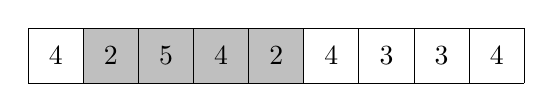
\begin{tikzpicture}[scale=0.7]
\fill[color=lightgray] (1,0) rectangle (5,1);
\draw (0,0) grid (9,1);
\node at (0.5, 0.5) {4};
\node at (1.5, 0.5) {2};
\node at (2.5, 0.5) {5};
\node at (3.5, 0.5) {4};
\node at (4.5, 0.5) {2};
\node at (5.5, 0.5) {4};
\node at (6.5, 0.5) {3};
\node at (7.5, 0.5) {3};
\node at (8.5, 0.5) {4};
\end{tikzpicture}
\end{center}
and the next range is
\begin{center}
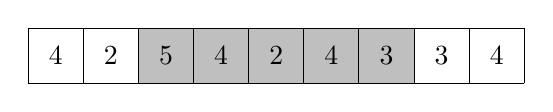
\begin{tikzpicture}[scale=0.7]
\fill[color=lightgray] (2,0) rectangle (7,1);
\draw (0,0) grid (9,1);
\node at (0.5, 0.5) {4};
\node at (1.5, 0.5) {2};
\node at (2.5, 0.5) {5};
\node at (3.5, 0.5) {4};
\node at (4.5, 0.5) {2};
\node at (5.5, 0.5) {4};
\node at (6.5, 0.5) {3};
\node at (7.5, 0.5) {3};
\node at (8.5, 0.5) {4};
\end{tikzpicture}
\end{center}
there will be three steps:
the left endpoint moves one step to the right,
and the right endpoint moves two steps to the right.

After each step, the array \texttt{count}
needs to be updated.
After adding an element $x$,
we increase the value of 
$\texttt{count}[x]$ by 1,
and if $\texttt{count}[x]=1$ after this,
we also increase the answer to the query by 1.
Similarly, after removing an element $x$,
we decrease the value of 
$\texttt{count}[x]$ by 1,
and if $\texttt{count}[x]=0$ after this,
we also decrease the answer to the query by 1.

In this problem, the time needed to perform
each step is $O(1)$, so the total time complexity
of the algorithm is $O(n \sqrt n)$.